\documentclass[tikz,border=5pt]{standalone}
\usepackage[dvipsnames]{xcolor}
\usepackage{tikz}
\usetikzlibrary{arrows.meta,calc,positioning,bending,quotes}

\tikzset{
  gnode/.style={
    circle,
    draw=blue!50!black,
    fill=blue!12,
    minimum size=10mm,
    inner sep=0pt,
    font=\Large\bfseries
  },
  connection/.style={
    thick,
    ->,
    >=Latex
  },
  glabel/.style={
    draw=black!55,
    line width=0.3pt,
    fill=white,
    rounded corners=1.5pt,
    inner sep=3pt,
    outer sep=3pt
  },
  every edge quotes/.append style=glabel
}

\def\nodeSep{3cm}

\begin{document}
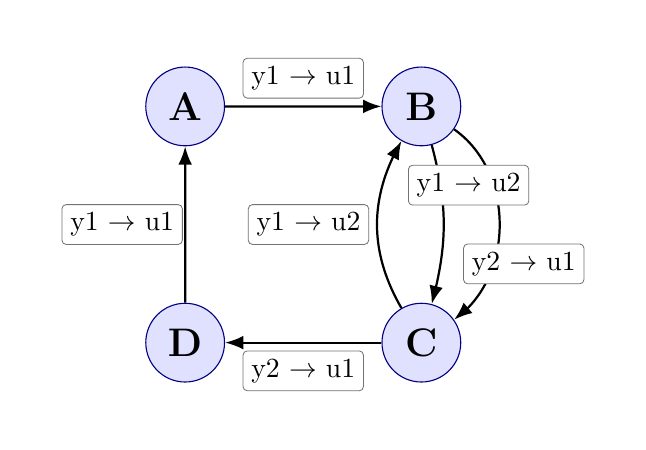
\begin{tikzpicture}
  % Force identical bounding box across all four panels
  \useasboundingbox (-1, -1) rectangle (6.5, 4);
  %\draw[help lines, step=0.5] (-1,-1) grid (6.5,4);

  \begin{scope}[xshift=1cm, yshift=0cm]
    % Nodes placed in the same 2x2 quadrants as the input-data panel
    \node[gnode] (A) at (0,\nodeSep)        {A};
    \node[gnode] (B) at (\nodeSep,\nodeSep) {B};
    \node[gnode] (D) at (0,0)               {D};
    \node[gnode] (C) at (\nodeSep,0)        {C};
    
    % A -> B, quotes auto-label
    \draw[connection] (A) edge[bend left=0, "y1 $\rightarrow$ u1"] (B);

    % Two parallel B -> C arcs, labels as explicit nodes so they sit on their own arc
    \draw[connection] (B) edge[bend left=15] (C);
    \draw[connection] (B) edge[bend left=55] (C);
    \node[glabel] at (3.6, 2) {y1 $\rightarrow$ u2}; % inner arc, upper half
    \node[glabel] at (4.3, 1) {y2 $\rightarrow$ u1}; % outer arc, lower half

    % C -> B on the opposite side of the B-C axis
    \draw[connection] (C) edge[bend left=30, "y1 $\rightarrow$ u2"] (B);

    % C -> D, quotes auto-label
    \draw[connection] (C) edge[bend left=0, "y2 $\rightarrow$ u1"] (D);

    % D -> A, label as explicit node to avoid overlap with the C-D arc
    \draw[connection] (D) edge[bend left=0] (A);
    \node[glabel] at (-0.8, \nodeSep/2) {y1 $\rightarrow$ u1};
  \end{scope}
\end{tikzpicture}
\end{document}
